
C++20对现有的并发性进行了增强,但我们将重点关注新添加的特性:协程。协程具有中断和恢复功能的线程,在几种主要的应用程序中很有用:可以极大地简化事件驱动程序的编写,对于窃取工作的线程池来说,那必然要使用协程,而且会让异步I/O和其他异步的代码更加简单

\subsubsubsection{8.4.1\hspace{0.2cm}介绍协程}

协同程序有两种风格:\textbf{有栈}和\textbf{无栈}。有栈协程有时也被称为\textbf{纤程}(fiber),类似于在堆栈上分配状态的函数。无栈协程没有相应的堆栈,状态存储在堆中。通常,有栈协程更加强大和灵活,但是无栈协程会更高效。

本书中,我们将重点关注无栈协程,因为C++20支持。这是一个不寻常的概念,在展示C++特有的语法和示例之前,先来解释一下。

常规的C++函数总是有一个相应的堆栈框架。只要函数在运行,栈帧就存在,所有的局部变量和其他状态都存储在这里。下面是一个简单的函数\texttt{f()}:

\begin{lstlisting}[style=styleCXX]
void f() {
	…
}
\end{lstlisting}

其中有一个栈帧。再函数\texttt{f()}调用另一个函数\texttt{g()}时:

\begin{lstlisting}[style=styleCXX]
void g() {
	…
}
void f() {
	…
	g();
	…
}
\end{lstlisting}

函数\texttt{g()}在函数运行时也有一个栈帧。 

参考下图:

%\hspace*{\fill} \\ %插入空行
\begin{center}
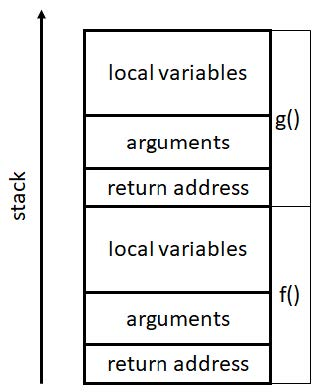
\includegraphics[width=0.6\textwidth]{content/2/chapter8/images/5.jpg}\\
图8.5 - 常规函数的栈帧
\end{center}

当函数\texttt{g()}退出时,它的栈帧会销毁,只有函数\texttt{f()}的栈帧保留了下来。

相反,无栈协程的状存储在堆上:这种分配称为\textbf{活帧}。活帧与协程句柄相关联,协程句柄是一个智能指针的对象。可以发出和返回函数的调用,只要句柄没有损坏,活帧就一直存在。

协程还需要堆栈空间,比如调用其他函数。该空间在调用者的堆栈上分配。下面是它的工作原理(C++语法有所不同,所以现在把协程相关的行为想象成伪代码):

\begin{lstlisting}[style=styleCXX]
void g() {
	…
}
void coro() { // coroutine
	…
	g();
	…
}
void f() {
	…
	std::coroutine_handle<???> H; // Not the real syntax
	coro();
	…
}
\end{lstlisting}

对应的内存分配如下图所示:

%\hspace*{\fill} \\ %插入空行
\begin{center}
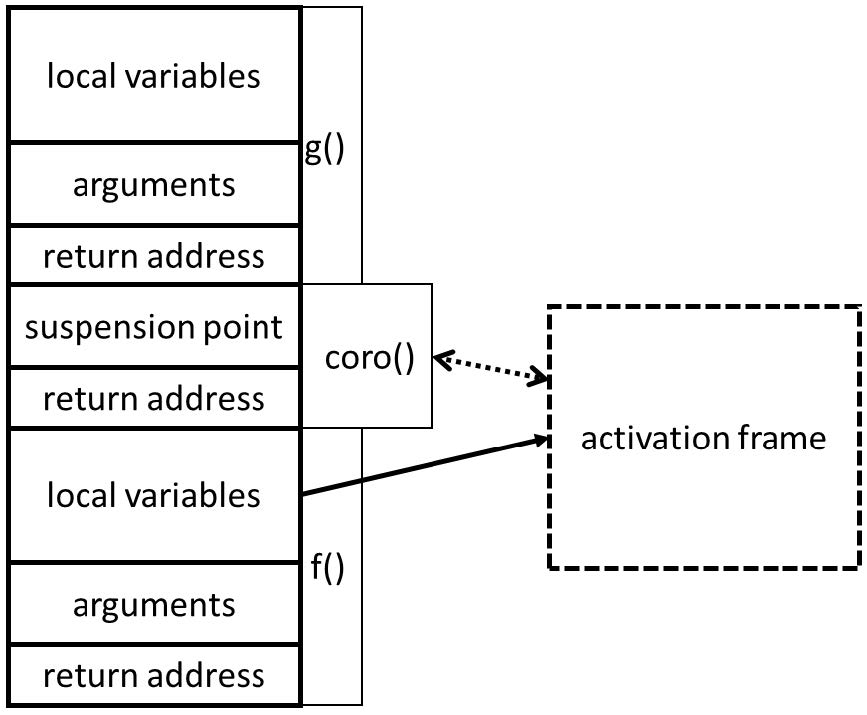
\includegraphics[width=0.6\textwidth]{content/2/chapter8/images/6.jpg}\\
图8.6 - 调用协程
\end{center}

函数\texttt{f()}创建协程句柄,所以拥有活帧。然后调用协程函数\texttt{coro()}。这时有一些堆栈分配,协程在堆栈上存储了在挂起时返回的地址(记住,协程是可以挂起自己的函数)。协程可以调用另一个函数\texttt{g()},将\texttt{g()}的栈帧分配到堆栈上。此时,协程不能再挂起:只有协程顶层函数可以挂起。函数\texttt{g()}无论谁调用最终都会返回,以同样的方式运行,这将破坏它的栈帧。协程现在可以挂起自己了,所以我们假设它挂起了。 

这是有栈协程和无栈协程的关键区别:有栈协程可以在函数调用任意深度的地方挂起,并将从那里恢复。但是这种灵活性需要很高的内存成本,尤其是运行时成本:无栈协程由于其有限的状态,效率要高很多。

当协程挂起时,恢复协程所需的部分状态会存储在活帧中。然后销毁协程的栈帧,并将控制权返回给调用者,直至协程调用的位置。如果协程完成,也会发生同样的情况,但是调用者有一种方法可以查询协程的状态是挂起还是完成。

调用者继续执行他的操作,并可以使用其他函数:

\begin{lstlisting}[style=styleCXX]
void h() {
	…
}
void coro() {…} // coroutine
void f() {
	…
	std::coroutine_handle<???> H; // Not the real syntax
	coro();
	h(); // Called after coro() is suspended
	…
}
\end{lstlisting}

内存分配看起来如下所示:

%\hspace*{\fill} \\ %插入空行
\begin{center}
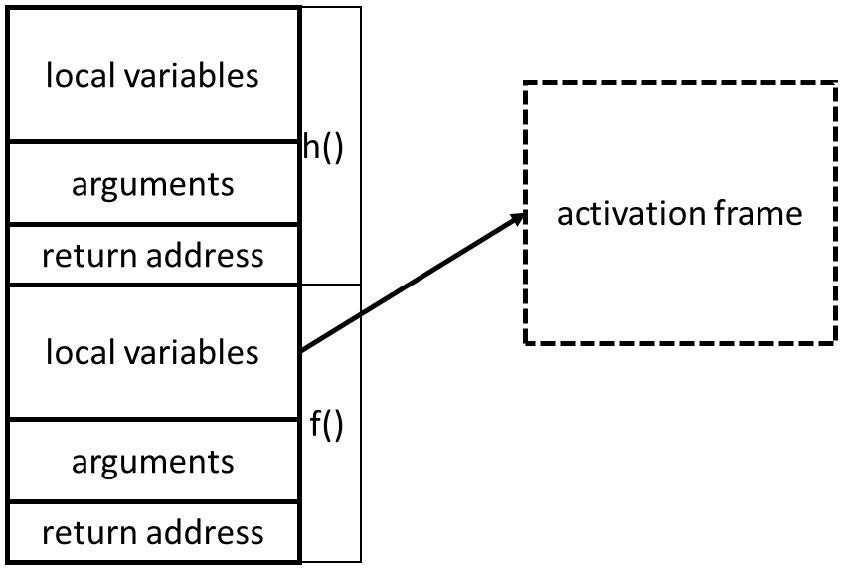
\includegraphics[width=0.6\textwidth]{content/2/chapter8/images/7.jpg}\\
图8.7 - 挂起协程,继续执行
\end{center}

注意,没有与协程对应的栈帧,只有堆分配的活帧。只要句柄对象处于活动状态,协程就可以恢复。不一定是调用和恢复协程的同一函数,例如:如果句柄可用,函数\texttt{h()}就可以恢复:

\begin{lstlisting}[style=styleCXX]
void h(H) {
	H.resume(); // Not the real syntax
}
void coro() {…} // coroutine
void f() {
	…
	std::coroutine_handle<???> H; // Not the real syntax
	coro();
	 h(H); // Called after coro() is suspended
	…
}
\end{lstlisting}

协程从暂停的地方重新开始,状态从活帧中恢复,任何必要的堆栈分配将像往常一样:

%\hspace*{\fill} \\ %插入空行
\begin{center}
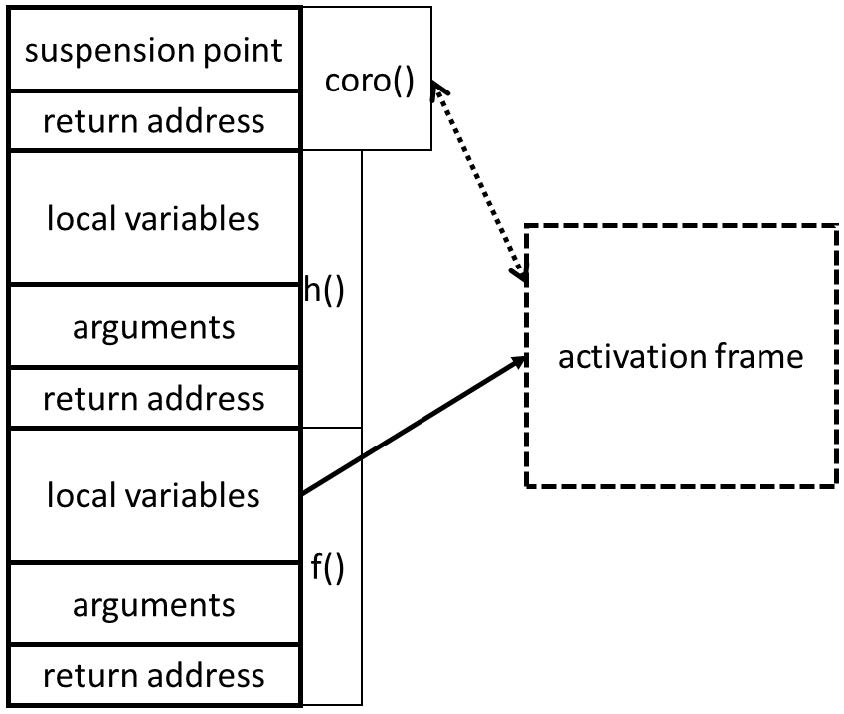
\includegraphics[width=0.6\textwidth]{content/2/chapter8/images/8.jpg}\\
图8.8 - 协程从不同的函数处恢复
\end{center}.

最终,协程完成,句柄销毁。这将释放与协程关联的所有内存。

以下是关于C++20协程需要了解的主要内容:

\begin{itemize}
\item
协程是可以挂起自己的函数。这与操作系统挂起一个线程不同:挂起一个协程是由开发者显式地完成的(多任务协作)。

\item
与栈帧相关联的常规函数不同,协程具有句柄对象。只要句柄处于活动状态,协程状态就会保持。

\item
协程挂起后,控制权将返回给调用者,调用者可以继续以相同的方式运行,就像协程已经完成一样。 

\item 
协程可以从任何位置恢复,不一定是调用者本身。此外,协程甚至可以从不同的线程恢复(将在本节后面看到一个示例)。协程从挂起点恢复,并继续运行,就像什么都没发生一样(但可能在不同的线程上运行)。
\end{itemize}

现在让我们了解一下所有这些在C++中是如何完成的。

\subsubsubsection{8.4.2\hspace{0.2cm}协程的C++语法}

现在让我们看一下C++语言的构造,这些构造可用于协程编程。 

首先,是获得一个支持该特性的编译器。GCC和Clang在他们的最新版本中都支持协程,但不幸的是,方式不同。对于GCC您需要版本11或更高版本。对于Clang,在版本10中添加了部分支持,并在以后的版本中进行了加强,但仍然是“实验性的”。

首先,为了编译协程代码,您需要在命令行上有一个编译器选项(使用\texttt{-std=c++20}选项启用C++20还不够)。对于GCC,这个选项是\texttt{-fcoroutines}。对于Clang,选项是\texttt{-stdlib=libc++ -fcoroutines-ts}。最新版的Visual Studio只需要\texttt{/std:c++20},不需要其他选项。

然后,需要包含协程头文件。在GCC和Visual Studio中(根据标准),头文件是\texttt{\#include <coroutine>},声明的所有类都在标准命名空间\texttt{std}中。但在Clang中,头文件是\texttt{\#include <experimental/coroutine>},使用的命名空间是\texttt{std::experimental}。

声明协程不需要特殊的语法,协程只是普通的C++函数。使它们成为协程的是使用暂停操作\texttt{co\_await}或其\texttt{co\_yield}。然而,在函数体中调用这些操作是不够的,C++中的协程对其返回类型有严格的要求。标准库在声明这些返回类型和其他处理协程所需的类时,没有提供任何帮助。语言仅提供了一个使用协程进行编程的框架。因此,直接使用C++20协程代码会非常冗长、重复,并且包含大量样板代码。实际中,每个使用协程的开发者都会使用一个可用的协程库。 

对于实际的编程,也应该这样做。本书中,我们将展示用简单的C++编写的示例。这样做的目的是,不想引入任何特定的库,而且这样做会模糊读者对实际情况的理解。对协程的支持是最近才出现的,这些库也在迅速发展,现在选择的库不一定会一直好用。我们希望在C++的级别理解协程代码,而不是在某个特定库所呈现的抽象级别理解协程代码。然后,应该根据自己的需要选择一个库,并使用它的抽象语法进行编程。

对与协程相关语法结构的全面描述非常不直观:它是一个框架,而不是一个库。出于这个原因,我们将使用示例来完成余下的演示。如果真的想知道协程的所有语法要求,必须查找最新的出版物(或阅读标准)进行了解。但是这些例子应该能对协程的功能有足够的展示,也可以阅读相关协程库的文档,并在程序中使用这个协程库。

\subsubsubsection{8.4.3\hspace{0.2cm}协程用例}

第一个例子是C++中协程最常见的用法(标准为协程提供了一些显式设计的语法)。我们将实现一个惰性生成器。生成器是生成数据序列的函数。每次调用生成器,都会得到序列的一个新元素。惰性生成器是按需计算元素的生成器。

下面是一个基于C++20协程的惰性生成器:

\hspace*{\fill} \\ %插入空行
\noindent
\textbf{coroutines\_generator1.C}
\begin{lstlisting}[style=styleCXX]
generator<int> coro(){
	for (int i = 0;; ++i) {
		co_yield i;
	}
}
int main() {
	auto h = coro().h_;
	auto& promise = h.promise();
	for (int i = 0; i < 3; ++i) {
		std::cout << "counter: " << promise.value_ << 
		std::endl;
		h();
	}
	h.destroy();
}
\end{lstlisting}

这是底层的C++代码,我们可以对其中涉及的每一步进行解释。首先,协程\texttt{coro()}看起来像个函数,\texttt{co\_yield}操作符除外。此操作符挂起协程,并将值\texttt{i}返回给调用者。因为协程挂起,而不是终止,所以操作符可以执行多次。和其他函数一样,协程在控件到达右大括号时终止。此时,无法恢复。通过\texttt{co\_return}(不应该使用常规的\texttt{return}),可以在退出协程。

其次,协程的返回类型——生成器——是需要定义的一种特殊类型。它有很多要求,这会导致了冗长的样板代码(任何协程库都预定义了这样的类型)。我们已经看到生成器包含一个嵌套的数据成员\texttt{h\_},而这就是协程句柄。这个句柄的创建也会创建活帧。句柄与\texttt{promise}对象关联,这与C++11的\texttt{std::promise}没有任何关系。事实上,它根本不是标准类型之一:我们必须根据标准中列出的一组规则来定义它。执行结束时,句柄会销毁,这也会销毁协程的状态。因此,句柄类似于指针。

最后,句柄是一个可调用对象。调用会恢复协程,因为\texttt{co\_yield}操作符在循环中,所以协程会生成下一个值,并立即再次挂起自己。 

通过为协程定义适当的返回类型,所有这些都可以神奇地结合在一起。就像STL算法一样,整个系统都受到规则的约束:这个过程中涉及到的所有类型都有期望,如果这些期望没有得到满足,那么就无法编译。现在来看看生成器的类型:

\begin{lstlisting}[style=styleCXX]
template <typename T> struct generator {
	struct promise_type {
		T value_ = -1;
		generator get_return_object() {
			using handle= std::coroutine_handle<promise_type>;
			return generator{handle::from_promise(*this)};
		}
		std::suspend_never initial_suspend() { return {}; }
		std::suspend_never final_suspend() noexcept { return 
			{}; }
		void unhandled_exception() {}
		std::suspend_always yield_value(T value) {
			value_ = value;
			return {};
		}
	};
	std::coroutine_handle<promise_type> h_;
};
\end{lstlisting}

首先,返回类型不必从模板生成,我们可以声明一个整数生成器。通常,是对生成序列中的元素类型参数化的模板。其次,命名生成器没有任何特殊之处,可以随意调用该类型(大多数库都提供了类似的模板,并将其称为生成器)。另一方面,嵌套类型\texttt{generator::promise\_type}必须称其为\texttt{promise\_type},否则,程序将无法编译。通常,嵌套类型本身命名成其他类型,并在使用时,使用类型别名:

\begin{lstlisting}[style=styleCXX]
template <typename T> struct generator {
	struct promise { … };
	using promise_type = promise;
};
\end{lstlisting}

\texttt{promise\_type}类型\textit{必须}是\texttt{generator}类的嵌套类型(或者,协程返回的类型)。但是\texttt{promise}类不强制是嵌套类:通常,它是嵌套类,但可以在外部进行声明。 

制性是需要\texttt{promise}类型的成员函数集合,包括签名。注意,有些成员函数是\texttt{noexcept}的。这也是需求的一部分:如果忽略此规范,程序将无法编译。当然,即使函数不会抛出异常,也没必要将其声明为\texttt{noexcept}。 

对于不同的生成器,这些必需的函数实现可能更加复杂。我们将简要描述他们的工作。

第一个非空函数\texttt{get\_return\_object()}是样板代码的一部分,看起来和前面的那个完全一样,这个函数从句柄构造了一个新的生成器,而句柄又是由\texttt{promise}对象构造的。编译器使用它,以获得协程的结果。 

第二个非空函数\texttt{yield\_value()},在每次使用操作符\texttt{co\_yield}时调用,它的参数是\texttt{co\_yield}值。将值存储在\texttt{promise}对象中,是协程将结果传递给调用者的常用方式。 

编译器在第一次遇到\texttt{co\_yield}时调用\texttt{initial\_suspend()}。\texttt{final\_suspend()}在协程通过\texttt{co\_return}生成最后一个结果后调用,之后不能暂停。如果协程结束时没有返回\texttt{co\_return},则调用\texttt{return\_void()}。最后,如果协同程序抛出了一个从其主体中逃逸的异常,则调用\texttt{unhandled\_exception()}。尽管些情况很罕见,使用者可以定制这些方法来特殊处理其中每一种情况。

现在我们来看看它们是如何结合在一起,为我们提供一个惰性生成器的。首先,创建协程句柄。在示例中,我们不保留生成器对象,只保留句柄。这不是必需的:可以保留生成器对象,并在其析构函数中销毁句柄。协程一直运行,直到遇到\texttt{co\_yield}挂起自己,控制权返回给调用者,而\texttt{co\_yield}的返回值在\texttt{promise}中捕获。调用程序获取此值,并通过调用该句柄恢复协程。协程从它挂起开始,一直运行到下一个\texttt{co\_yield}。 

我们的生成器可以永远运行(或者达到平台上的最大整数值),流程永远不会结束。如果需要一个有限长度的序列,可以执行\texttt{co\_return},或在流程结束后退出循环。参考以下代码:

\begin{lstlisting}[style=styleCXX]
generator<int> coro(){
	for (int i = 0; i < 10; ++i) {
		co_yield i;
	}
}
\end{lstlisting}

现在我们有一个10个元素的序列。在尝试恢复协程之前,调用者必须检查句柄成员函数\texttt{done()}的结果。

我们在前面提到过,可以从代码中的任何地方恢复协程(当然是在它挂起后),甚至可以从不同的线程恢复。这种情况下,协程开始在一个线程上执行和挂起,然后在另一个线程上运行它的其余代码。让我们看一个例子:

\hspace*{\fill} \\ %插入空行
\noindent
\textbf{coroutines\_change\_threads.C}
\begin{lstlisting}[style=styleCXX]
task coro(std::jthread& t) {
	std::cout << "Coroutine started on thread: " <<
		std::this_thread::get_id() << '\n';
	co_await awaitable{t};
    std::cout << "Coroutine resumed on thread: " <<
		std::this_thread::get_id() << '\n';
	std::cout << "Coroutine done on thread: " <<
		std::this_thread::get_id() << '\n';
}
int main() {
	std::cout << "Main thread: " <<
		std::this_thread::get_id() << '\n';
	std::jthread t;
	coro(t);
	std::cout << "Main thread done: " << 
		std::this_thread::get_id() << std::endl;
}
\end{lstlisting}

首先,让我们了解一些细节信息:\texttt{std::jthread}在C++20中添加,它只是一个可汇入的线程——它会连接到对象的析构函数中(几乎所有使用线程的人都为此编写了一个类,但现在有了一个标准的类)。现在我们可以来看看最重要的部分——协程本身。 

了解一下协程的返回类型:

\begin{lstlisting}[style=styleCXX]
struct task{
	struct promise_type {
		task get_return_object() { return {}; }
		std::suspend_never initial_suspend() { return {}; }
		std::suspend_never final_suspend() noexcept { return 
			{}; }
		void return_void() {}
		void unhandled_exception() {}
	};
};
\end{lstlisting}

这可能是协程的最小返回类型:包含所有必需的样板,而不包含其他内容。具体来说,返回类型是一个嵌套类型\texttt{promise\_type}类。该嵌套类型必须定义几个成员函数,如下面的代码所示。前面示例中的生成器类型包含这些内容,以及用于将结果返回给调用者的数据。当然,任务也可以根据需要具有内部状态。

与前面的例子相比,第二个变化是任务挂起的方式:我们使用\texttt{co\_await},而不是\texttt{co\_yield}。操作符\texttt{co\_await}实际上是挂起协程的更通用的方法:就像\texttt{co\_yield}一样挂起函数,并将控制权返回给调用者。区别在于参数类型:\texttt{co\_yield}返回一个结果,而\texttt{co\_await}的参数是一个\texttt{waiter}对象。同样,对该对象的类型也有特定的要求。如果满足了这个要求,类就可称为\texttt{awaitable},这种类型的对象是一个有效的awaiter(如果不是,则无法编译)。以下是我们的\texttt{awaitable}:

\begin{lstlisting}[style=styleCXX]
struct awaitable {
	std::jthread& t;
	bool await_ready() { return false; }
	void await_suspend(std::coroutine_handle<> h) {
		std::jthread& out = t;
		out = std::jthread([h] { h.resume(); });
	}
	void await_resume() {}
	~awaitable() {}
	awaitable(std::jthread& t) : t(t) {}
};
\end{lstlisting}

\texttt{awaitable}所需的接口是这里的三个函数。第一个是\texttt{await\_ready()}:它在协程挂起后调用。如果返回true,那么协程的结果就准备好了,并且没有必要挂起协程。实际中,这个函数总是返回false,这将导致协程的暂停:协程的状态,例如局部变量和暂停点,都存储在活帧中,控制权返回给调用者或恢复者。第二个函数是\texttt{await\_resume()},在协程恢复后继续执行之前调用。如果它返回结果,那就是整个\texttt{co\_await}操作符的结果(我们的例子中是没有结果的)。最有趣的函数是\texttt{await\_suspend()},它在当前协程挂起时,使用当前协程的句柄进行调用,并且可以有几种不同的返回类型和值。如果它返回void(正如在我们的示例中所做的那样),协程将挂起,控制权将返回给调用者或恢复者。不要被我们示例中的\texttt{await\_suspend()}所迷惑:它不会恢复协程。相反,它创建一个将执行可调用对象的新线程,并且正是这个对象恢复了协程。协程可以在\texttt{await\_suspend()}完成,或仍在运行时恢复:这个例子演示了异步操作时协程的用法。 

把所有这些放在一起,我们得到这个流程:

\begin{enumerate}
\item
主线程调用协程。

\item
操作符\texttt{co\_await}挂起协程。这个过程涉及到对\texttt{awaitable}对象成员函数的调用,其中一个调用会创建一个新线程,其会恢复协程(带有移动分配线程对象的游戏已经结束,所以我们删除了主程序中的新线程,这样可以避免了一些糟糕的竞争条件)。

\item
控制权返回给协程的调用方,因此主线程在协程调用之后继续从该行运行。如果线程在协程完成之前到达那里,将在线程对象\texttt{t}的析构函数中进行阻塞。

\item 
新线程会恢复协程,并从\texttt{co\_await}之后的行继续在该线程上执行。由\texttt{co\_await}构造的\texttt{awaitable}对象会销毁。协程运行到最后,全部在第二个线程上运行。到达协程的末尾意味着它完成了,就可以汇入运行协程的线程了。若主线程正在等待线程\texttt{t}的析构函数完成,现在则会解除阻塞,并汇入线程(如果主线程还没有到达析构函数,那么当它到达析构函数时就不会阻塞)。
\end{enumerate}

该流程可以通过程序的输出进行确认:

\begin{tcblisting}{commandshell={}}
Main thread: 140003570591552
Coroutine started on thread: 140003570591552
Main thread done: 140003570591552
Coroutine resumed on thread: 140003570587392
Coroutine done on thread: 140003570587392
\end{tcblisting}

如您所见,协程\texttt{coro()}首先在一个线程上运行,然后在执行过程中跳转到另一个线程。如果有任何局部变量,将在转换过程中保留。

我们提到\texttt{co\_await}是暂停协程的通用操作符。实际上,\texttt{co\_yield x}操作符等价于\texttt{co\_await}的特殊用法:

\begin{lstlisting}[style=styleCXX]
co_await promise.yield_value(x);
\end{lstlisting}

这里的\texttt{promise}是与当前协程句柄关联的\texttt{promise\_type}对象。使用操作符\texttt{co\_yield}的原因是,从协程内部访问自己的\texttt{promise}会出现相当复杂的语法使用,因此标准为其添加了一个快捷方式。

这些例子演示了C++协程的功能。协程最有用的功能是工作窃取(您已经看到将协程的执行转移到另一个线程是多么容易)、惰性生成器和异步操作(I/O和事件处理)。尽管如此,协程在C++中的时间还不够长,还没有形成使用模式,所以社区还没有提出使用协程的最佳实践。同样,现在谈论协程的性能还为时过早,我们必须等待编译器支持成熟的和更大规模的应用程序开发。 

总的来说,在多年忽视并发性之后,C++标准正在迅速赶上,所以让我们总结一下语言最近的进展。









